%   MSc Business Analytics Dissertation
%
%   Title:     Aaa Bbbbbbb Cccccccccc
%   Author(s): Xxxxxx Xxxxxxxxx and Yyy Yyyyyyyyy
%
%   Chapter 4: Methodology
%
%   Change Control:
%   When     Who   Ver  What
%   -------  ----  ---  --------------------------------------------------------------
%   11Feb11  AB    0.1  Begun 
%

\chapter{Methodology}\label{C.Methodology}

\section{Overview}\label{S.Ch4.opening}
To assist financial auditor or stakeholder at financial institutions and banks, and to identify such loan portfolio which may default in future based on the geospatial information and financial data. This research work followed the KDD process which involves characteristics variables selection, perform data restructuring, data transformation and data mining for the deployment of a predictive model using visual analytics tools such as Tableau, QlikView, etc.

\textbf{Software \& Tools used:}

Following is the list of tools and softwares that has been used while working on this project:
\begin{description}
  \item[Data Processing:] MS Excel 2017 and Alteryx Desginer 11.0
  \item[Version Control:] Github (github.com)
  \item[Dashboard:] Tableau Professional 10.2 and R Stuio 1.0.36
  \item[Data Storage:] Github Pages (https://pages.github.com/) and Google Drive
\end{description}
\textbf{R Packages used:}
\begin{description}
  \item[Packages required Logisctic Regression Model:] Following packages used to building simple regression and logistic regression based model for predictig the good or bad loan portfolio: glm() with class set to "bionomial" for Logistic Regression and "log" for Poisson regression, ROSE, ROCR, Dplyr, maps, ggplot2
  \item[Decession Tree:] Following r-packages used for building a predictive model based on decision tree: caret, rpart, rattle, ROSE, ROCR, RColorBrewer, party, partykit
\end{description}
\textbf{R Shiny:} R Shiny packages for building interactive dashboards: leaflet, maps, ggmap, gridExtra, htmlwidgets, reshape2. To deploy predictive model on Tableau to build dyanmic and easy to user dashboard R Server used


One may replicate our work on his/her computer having minimum hardware specifications outlined here. This research work carried on following machines. 

% \usepackage{booktabs}
\begin{table}[!htb]
\centering
\caption{System configurations used to carry out this research}
\label{osc4}
\begin{tabular}{|p{3cm}|p{5cm}|p{5cm}|}
\toprule
\textbf{Specification}    & \textbf{System 1 - Lenovo Yoga 500}   & \textbf{System 2 - Dell Inspiron 15} \\ \midrule
\textbf{Operating System} & Windows 10 Professional               & Windows 7 Professional               \\
\textbf{Processor}        & Intel(R) Core(TM) i3-5005CU @ 2.00GHz & Intel(R) Core(TM) i3-3217U @ 1.80GHz \\
\textbf{RAM}              & 4.00 GB                               & 4.00 GB                              \\
\textbf{System Type}      & 64-bit OS, x64-Based Processor        & 32 -bit Operating System             \\ \bottomrule
\end{tabular}
\end{table}


\section{Data Processing \& Analysis}\label{ch4.3}

\subsection{Overview}
One requires the accessibility to the right set of data, and information on which statistical and modelling techniques can be applied to start any data oriented research in analytics domain, KPMG, Ireland provided data set. This data set contains historical data of various loan portfolios that maintained by each branch of banks or financial institutions. Also, this dataset has geospatial information about credit account along with their transactional history of previous loans. Credit scoring model requires being trained with a correct set of characteristics variables to provide the prediction with high accuracy.\\

This project has been carried out in four stages as outlined below:
\begin{itemize}
  \item Data Selection \& Processing
  \item Model Design \& Implementation
  \item Testing \& Model Results
  \item Deployment \& Visualizations
\end{itemize}

\subsection{Data Set}
Dataset format: .xlsx\\
Number of attributes: 35\\
Total number of records: 237,390\\
All the variables and attributes have been carefully studied and analysed to decide what key factors will be used to develop the model. Based on the availability of RAM on the current system, it was decided to build a model on selected characteristics variables. One may train the model with all possible variables as well if system hardware allows. Below is the list of variables in original dataset:

\begin{verbatim}

[1] "ContractRef"           "LoanBalance"    "InterestType"    
[4] "ProbationaryLoans"     "MortgageType"   "NewLoan"         "NIM"  
[8] "DefaultedLoans"        "CreditRating"   "InterestIncome"  "LTV"               
[12] "LTVCategory"          "MortgageYears"  "PropertyValue"             
[15] "MaturityDate"         "BookingDate"    "LastValuationDate"      
[18] "County"               "Branch"         "Address"   
[21] "Town"                 "InArrears"      "AddressLongitude" 
[24] "AddressLatitude"      "DaysInArrears"  "ArrearsCategory"
[27] "HousePriceMovement"   "ValueInArrears" "ValuationAgeYears"
[30] "UpdatedPropertyValue" "LTVUpdated"     "LTVCategoryUpdated"
[33] "CreditRatingMovement" "InterestRate"   "AnnualPYMT"

\end{verbatim}

Below is the comprehensive list of all variables that have been chosen for the model creation:
\begin{description}
  \item[ContractRef]: Unique reference number assigned to each portfolio
  \item[InterestType]: There are three types of interest rate: Fixed, Tracker and Variable
  \item[MortgageType]: Whether property is bought for "buy-to-let" or "owner occpied"
  \item[NewLoan]: Is portfolio is new or existing?
  \item[ProbationaryLoans]: Has loan been taken on probation?
  \item[DefaultedLoans]: Classify if the loan has defaulted in the past
  \item[LTVCategory]: 5 Level categorized pre-assigned to each loan account
  \item[CreditRating]: Each account is rated from 1-5 scale on the basis of credit union policy
  \item[MortgageYears]: How many years mortgage has been taken for?
  \item[CreditRatingMovement]: Percentage that indicates how credit rating has moved from previous value for an application
  \item[LTV]: Ratio of applied loan amount to property evaluation value 
  \item[LoanBalance]: How much loan amount is left to repay?
  \item[InterestIncome]: How much interest amount bank is earning?
  \item[PropertyValue]: Recent property evaluation amount
  \item[AnnualPYMT]: How much amount is getting repaid to the bank by the applicant annually?
  \item[AddressLatitude]: Latitude value of the house on map
  \item[AddressLongitude]: Longiitude value of the house on map
  \item[County]: Name of the county where house is located
  \item[InArrears]: Any amount that has not been paid earlier on time
  \item[ArrearsCategory]: Category that defines duration of Arrears such as more than 90 days
\end{description}

\textbf{Structure of the Data}
\begin{verbatim}
Classes ‘tbl_df’, ‘tbl’ and 'data.frame':	36696 obs. of  20 variables:
 $ ContractRef         : chr  "00000CONTR00111034" "00000CONTR00146183"
    "00000CONTR00175040" "00000CONTR00171901" ...
 $ InterestType        : Factor w/ 3 levels "Fixed","Tracker",..:
    2 3 2 1 2 3 2 2 2 3 ...
 $ MortgageType        : Factor w/ 2 levels "Buy to Let",
     "Owner Occupied": 1 2 2 2 2 2 2 2 2 2 ...
 $ NewLoan             : Factor w/ 2 levels "No","Yes":
    1 1 1 1 1 1 1 1 2 1 ...
 $ ProbationaryLoans   : Factor w/ 2 levels "No","Yes": 
    2 1 1 1 1 1 1 1 1 1 ...
 $ DefaultedLoans      : Factor w/ 2 levels "No","Yes":
    2 2 2 2 2 2 2 2 2 2 ...
 $ LTVCategory         : Factor w/ 11 levels "> 100%","0 to 10%",..:
    11 8 11 5 3 5 9 11 9 9 ...
 $ CreditRating        : Factor w/ 5 levels "1","2","3","4",..:
    4 2 4 4 3 2 3 3 4 2 ...
 $ MortgageYears       : int  31 30 30 29 29 32 28 35 29 31 ...
 $ CreditRatingMovement: int  3 0 0 0 2 -3 0 0 0 0 ...
 $ LTV                 : num  0.983 0.65 0.93 0.368 0.167 ...
 $ LoanBalance         : num [1:36696, 1] -0.647 -0.297 1.418
    -0.986 -1.32 ...
  ..- attr(*, "scaled:center")= num -1.05e-17
  ..- attr(*, "scaled:scale")= num 1
 $ InterestIncome      : num [1:36696, 1] -0.71 -0.132 1.53 
    -0.203 -1.1 ...
  ..- attr(*, "scaled:center")= num -2.14e-17
  ..- attr(*, "scaled:scale")= num 1
 $ PropertyValue       : num [1:36696, 1] -1.3 -0.311 0.779
    -0.511 -0.205 ...
  ..- attr(*, "scaled:center")= num -2.51e-17
  ..- attr(*, "scaled:scale")= num 1
 $ AnnualPYMT          : num [1:36696, 1] -1.2756 -0.2211 
    0.9057 -0.3651 ...
  ..- attr(*, "scaled:center")= num 9.48e-18
  ..- attr(*, "scaled:scale")= num 1
 $ AddressLatitude     : num  52.4 53.3 52.8 53.7 53.4 ...
 $ AddressLongitude    : num  -7.7 -6.27 -6.74 -6.68 -6.21 ...
 $ InArrears           : Factor w/ 2 levels "No","Yes":
    1 1 1 1 1 1 1 2 1 2 ...
 $ County              : Factor w/ 26 levels "Carlow","Cavan",..: 
      22 6 1 17 6 9 16 22 6 6 ...
 $ ArrearsCategory     : chr  "0" "0" "0" "0" ...
\end{verbatim}

\section{Implementation}\label{}

\begin{figure}
\centering
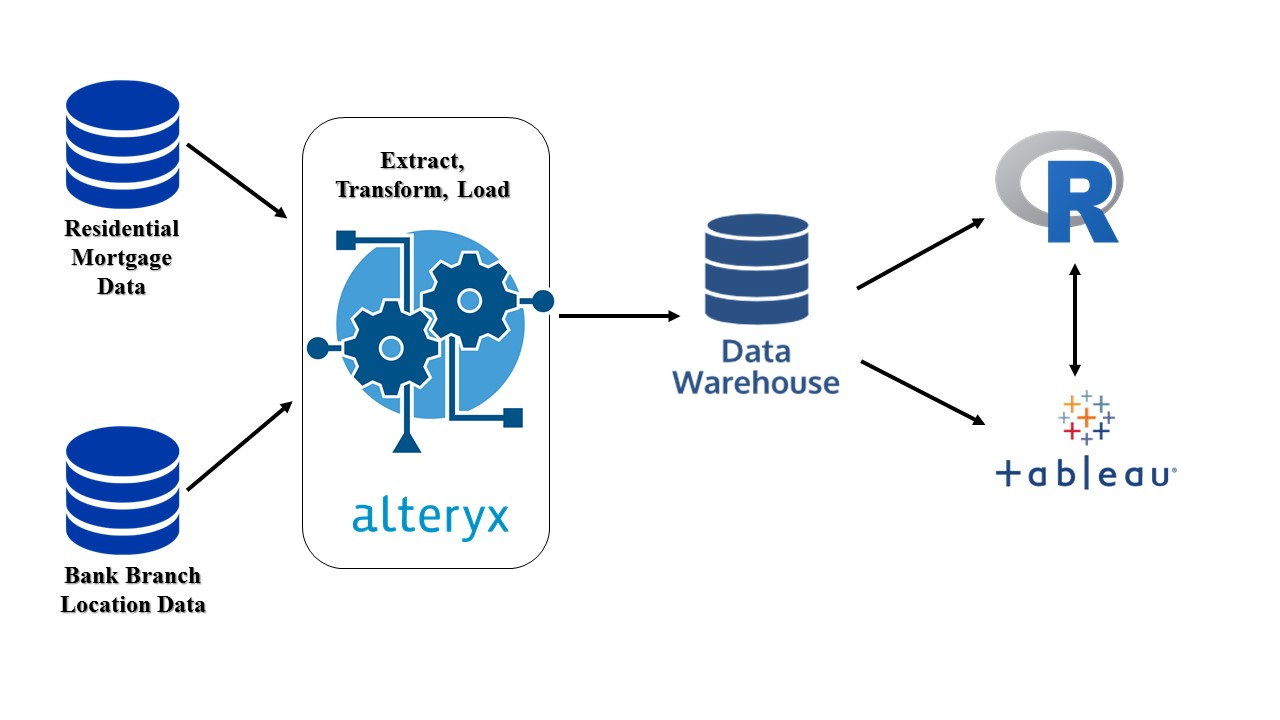
\includegraphics[width=\textwidth]{ETL.jpg}
\caption{ETL \& Data Model Architecture}{\textbf{Source}: Designed using MS Office}
\end{figure}


\subsection{Data Extraction} Prior building predictive model in R one, need to process and analyse the data. The primary objective is to identify any outliers and to normalise the available data set. \cite{sola1997importance}, observed that un-normalized data tends to increase square mean error and then deviate the model prediction. Therefore, it is important to treat data and normalised it's all variables so that model works with high precision and accuracy. One can also do data pre-processing using R as well, but Alteryx provides graphical user interface to select features and settings that makes whole data processing phase easy and fast\\

\textbf{Alteryx Desginer} tool allow one to build workflow to prepare data from multiple data sources on the go and by using features such as 'Select', 'Random Sample', 'Transform' and 'Output' one can easily prepare data for the predictive model \citep{dinsmore2016self}. Alteryx can process large amount of dataset and optimized it to be ready for data modelling in R.

\begin{center}
\begin{figure}[ht]
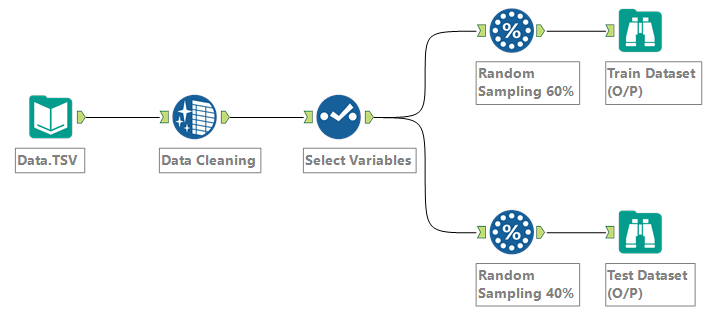
\includegraphics[width=\textwidth]{dataprocess.png}
\centering
\caption{Data Processing using Alteryx}{\textbf{Source:} Designed using in Alteryx Designer v11}
\label{fig:dataprocessing}
\end{figure}
\end{center}

In fig.\ref{fig:dataprocessing}, raw data has been read using \emph{Input tool}, then null values, white spaces etc removed using \emph{Cleansing Tool} and variables selection has been done using \emph{Select Tool}. To create train data set and test data set \emph{Random Sample \% tool}, which allows generating sample datasets.\\

\subsection{Data Transformation}
In Alteryx, there is no provision to normalize data. Processed data from Alteryx is loaded into \textbf{R Studio} for data normalization or scaling using in built functions such as scale($<variable>$) and log($<variable>$) on $LoanBalance$, $PropertyValue$, $InterestIncome$ and $AnnualPYMT$ as these variables are crucial paramters for credit scoring to make unbaised prediction model.\\

\textbf{R Studio}: Data from Alteryx is loaded to R Studio for the development of prediction model. R is used to identify patterns or correlation in variables using \emph{ggplot2}, \emph{plot.ly}, \emph{leaflets}. Two predictive models have developed based Logistic Regression and Decision Tree algorithms and both models performance evaluated concerning accuracy. Trained model is saved on the hard drive and loaded in Tableau, and with the help of R Server, Tableau allows the user to build dynamic visualizations. In Tableau, calculated fields can dynamically invokes R engine to perform calculations and then R results output values back to Tableau, so that visualizations can be designed.\\


\subsection{Data Loading}\label{tableau}
\textbf{Integration of R in Tableau}: Processed and transformed data is loaded into Tableau for building business dashboards. Credit analyst or auditors will use the dashboard to identify locations where the most number of loan default happenings or identify those portfolios which have provided incorrect information, etc. business decisions can be made with the help of credit scoring dashboard.\\

\textbf{Installtion of R Server:} Local instance of R Server is deployed by installing \emph{Rserve} package from R console. To invoke R Server with following command:
      \begin{verbatim}
      install.packages("Rserve")
      library(Rserve)
      Rserve()
      \end{verbatim}

\textbf{Setting in Tableau}:\\

In Tableau, go to \emph{Settings and Performance} under \emph{Help} menu and then select \emph{Manage External Service Connection}. Following settings are required to connect with R server:
      \begin{verbatim}
      Server: "localhost" or "127.0.0.1
      Port: 6311
      \end{verbatim}

R scripts are written in calculated fields of Tableau to make calls to R using in built functions in Tableau such as \emph{SCRIPT\_STR} and \emph{SCRIPT\_REAL}



\section{Predictive Model}

\subsection{Overview}
\cite{shmueli2011predictive}, define predictive analytics as the process of building statistical models using data mining algorithm with an objective to predict the outcome on future data set. A model is evaluated based on its predictive power or accuracy. As discussed in section \ref{c3.tech}, Logistic regression and Decision Tree are most commonly algorithms for building predictive models for credit scoring. Based on the requirement of predictive algorithms, data type of certain variables has been converted using below code:

\begin{verbatim}
Datav2$CreditRating <- as.factor(Datav2$CreditRating)
Datav2$InterestType <- as.factor(Datav2$InterestType)
Datav2$MortgageType <- as.factor(Datav2$MortgageType)
Datav2$NewLoan <- as.factor(Datav2$NewLoan)
Datav2$ProbationaryLoans <- as.factor(Datav2$ProbationaryLoans)
Datav2$LTVCategory <- as.factor(Datav2$LTVCategory)
Datav2$InArrears <- as.factor(Datav2$InArrears)
Datav2$County <- as.factor(Datav2$County)
Datav2$DefaultedLoans <- as.factor(Datav2$DefaultedLoans)
Datav2$LoanBalance <- scale(Datav2$LoanBalance)
Datav2$PropertyValue <- scale(Datav2$PropertyValue)
Datav2$InterestIncome <-scale(Datav2$InterestIncome)
Datav2$AnnualPYMT <-scale(Datav2$AnnualPYMT
\end{verbatim}

\subsection{Logistic Regression}

Logistic regression is the most commonly used technique in credit scoring as it works on binary response variables, i.e., 0 or 1 \citep{hilbe2011logistic}. In fig. \ref{fig:logistic}, output results of standard logistics regression function lies between 0 and 1 only. In this research work output of response variable, i.e., the probability of default $p=1$ is considered as 'Yes' and $p=0$ is considered as 'No'. Probability is represented using logistic function (logit) and the probability of binary response variable based on the one, or more independent variables.

\begin{center}
\begin{figure}[!htb]
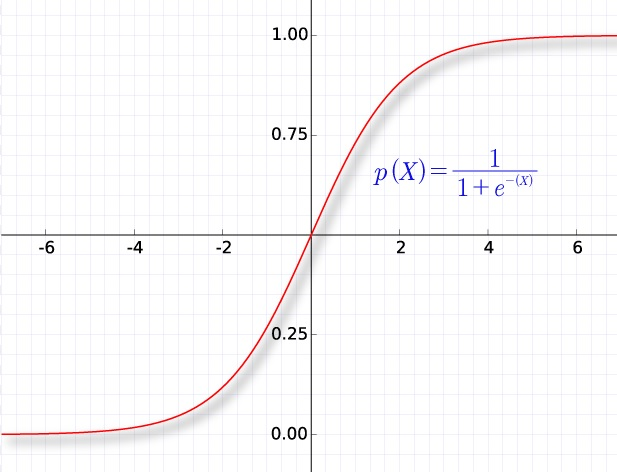
\includegraphics[width=\textwidth]{logistic.jpg}
\centering
\caption{Standard Logistic Regression}{\textbf{Source:} http://www.thefactmachine.com/wp-content/uploads/2015/03/13-Sigmoid.gif}
\label{fig:logistic}
\end{figure}
\end{center}

\subsubsection*{Model Settings:}
\textbf{Response Variable:} DefaultedLoans\\
\textbf{Family (Function):} "Binomial" (Logit)

\subsubsection*{Model Implementation Details:}
Initially, To train the model for all variables available in the dataset, but the model couldn't be trained because R engine failed to allocate 5.0GB vector space for the model. Following the line of code is used:

\begin{verbatim}
library(stats)
m2 <- glm(DefaultedLoans ~., family = "binomial", data = trainDatav2)
\end{verbatim}

Next, model is trained with selective variables set and following code is used:

\begin{verbatim}
simpleglmv2 <- glm(DefaultedLoans ~ CreditRating + InterestIncome + 
    log(PropertyValue) + log(LoanBalance) + AnnualPYMT + LTV + 
    InterestType + NewLoan + ProbationaryLoans + MortgageYears + 
    MortgageType + InArrears + County + AddressLatitude + AddressLongitude, 
    family = "binomial", data = trainDatav2)
\end{verbatim}

Trained model is used to predict output for test dataset using following code:
\begin{verbatim}
testDatav2$prediction <- predict(simpleglmv2, newdata=testDatav2,
type="response")
\end{verbatim}


\subsection{Decission Tree}

As discussed in section \ref{logit}, Decision Trees has two most commonly used algorithm for credit scoring i.e. CART and C4.5. Classification and regression trees (CART) has been implemented using rpart() package available in R to build predicive model. rpart() syntax is \begin{verbatim}
rpart(formula, data=, method=,control=)
\end{verbatim}

\begin{description}
  \item[formula =] DefaultedLoans ~ NewLoan + County + LoanBalance + PropertyValue + InterestIncome + CreditRating + AnnualPYMT + County + LTV + LTVCategory + InArrears + MortgageType + MortgageYears + AddressLatitude + AddressLongitude
  \item[data =]trainDatav2
  \item[method =] "Class"
  \item [control =] Parameters for controlling the growth of tree. \\
  \textbf{control =  rpart.control(minisplit=500,cp = 0.001))} At least 500 observations should be on a node before attempting a split and reduce the split fit factor by 0.001 before being attempted.
\end{description}

Packages such as rattle(), RColorBrewer(), etc. used to enhance the overall decision tree.

\subsubsection*{Model Implementation Details:}

\begin{verbatim}
library(rpart)
library(rattle)					# Fancy tree plot
library(rpart.plot)			# Enhanced tree plots
library(RColorBrewer)		# Color selection for fancy tree plot
library(party)					# Alternative decision tree algorithm
library(partykit)				# Convert rpart object to BinaryTree
library(caret)
defaultLoanTree <- rpart(DefaultedLoans ~ NewLoan + County + LoanBalance 
+ PropertyValue + InterestIncome + CreditRating + AnnualPYMT + County 
+ LTV + LTVCategory + InArrears + MortgageType + MortgageYears 
+ AddressLatitude + AddressLongitude ,method = "class",data=trainDatav2,
control =  rpart.control(minisplit=5,cp = 0.001))

save(fit, file = "Model/classificationTreeV2.rda")
print(defaultLoanTree)
prp(defaultLoanTree)
tree.1 <- defaultLoanTree
fancyRpartPlot(tree.1)
\end{verbatim}

Finally, Model performance of logistic regression and decision tree has been evaulated based on GINI, ROC metrics.

\section{Tableau \& Dashboards} 

Tableau professional software is used to develop the business dashboard that will be utilised by end users such as credit analyst, auditors, banks officials, etc. In Tableau, CSV file connector is used to connect to the data source ( sample dataset); then it is used to prepare various graphs and geospatial dashboard. Calculated field in Tableau allows making the call to R engine directly. By using calculated field options in Tableau, the predictive model is loaded into Tableau to make direct calls to R engine. Instructions and settings mentioned in section \ref{tableau} used as is to connect Tableau with R. \\

In the dashboard, the user can select an origin city or region and distance (in miles) from that origin. Based on these inputs user will be able to take the business decision such as investigating a loan account when property value of a particular house is higher than the area average property value, or opening new branches near by to areas for which a high number of loan applications is coming in. Following calculations are performed in Tableau calculated fields:

\textbf{Calculation for distance from Origin city}:
\begin{verbatim}
3959 * ACOS
(
  SIN(RADIANS(LOOKUP(AVG([Address Latitude]), First()))) * 
  SIN(RADIANS(AVG([Address Latitude]))
) +
  COS(RADIANS(LOOKUP(AVG([Address Latitude]), First()))) * 
  COS(RADIANS(AVG([Address Latitude]))) 
  * COS(RADIANS(AVG([Address Longitude])) - 
  RADIANS(LOOKUP(AVG([Address Longitude]),
  First())))
)
\end{verbatim}


\textbf{Calculation script for logistic regression model in Tableau:}
\begin{verbatim}
SCRIPT_REAL('mydata <- data.frame(DefaultedLoans=.arg1, CreditRating=.arg2,
InterestIncome=.arg3, LoanBalance =.arg4, AnnualPYMT =.arg5, LTV =.arg6,
InterestType=.arg7,NewLoan=.arg8, ProbationaryLoans = .arg9, 
MortgageYears=.arg10,MortgageType=.arg11, InArrears =.arg12,County =.arg13,
AddressLatitude=.arg14, AddressLongitude=.arg15, PropertyValue=.arg16);
load("Model/simpleglmv2.rda")

prob <- predict(simpleglmv2, newdata = mydata, type = "response")',
ATTR([Defaulted Loans]),ATTR([Credit Rating]),AVG([Interest Income]),
AVG([Loan Balance]),AVG([Annual PYMT]),AVG([LTV]),ATTR([Interest Type]),
ATTR([New Loan]),ATTR([Probationary Loans]),AVG([Mortgage Years]),
ATTR([Mortgage Type]),ATTR([In Arrears]),ATTR([County]),
AVG([Address Latitude]),AVG([Address Longitude]),AVG([Property Value]))
\end{verbatim}




